%%%%%%%%%%%%%%%%%%%%%%%%%%%%%%%%%%%%%%%%%%%%%%%%%%%%%%%%%%%%%%%%%%%%%%%%%%%%%%%%
%2345678901234567890123456789012345678901234567890123456789012345678901234567890
%        1         2         3         4         5         6         7         8

\documentclass[letterpaper, 10 pt, conference]{ieeeconf}  % Comment this line out
                                                          % if you need a4paper
%\documentclass[a4paper, 10pt, conference]{ieeeconf}      % Use this line for a4
                                                          % paper

\IEEEoverridecommandlockouts                              % This command is only
                                                          % needed if you want to
                                                          % use the \thanks command
\overrideIEEEmargins
% See the \addtolength command later in the file to balance the column lengths
% on the last page of the document



% The following packages can be found on http:\\www.ctan.org
\usepackage{graphics} % for pdf, bitmapped graphics files
\usepackage{epsfig} % for postscript graphics files
%\usepackage{mathptmx} % assumes new font selection scheme installed
%\usepackage{times} % assumes new font selection scheme installed
%\usepackage{amsmath} % assumes amsmath package installed
%\usepackage{amssymb}  % assumes amsmath package installed

\title{\LARGE \bf
BusBot: An Approach Towards Learning Stains
}

%\author{ \parbox{3 in}{\centering Huibert Kwakernaak*
%         \thanks{*Use the $\backslash$thanks command to put information here}\\
%         Faculty of Electrical Engineering, Mathematics and Computer Science\\
%         University of Twente\\
%         7500 AE Enschede, The Netherlands\\
%         {\tt\small h.kwakernaak@autsubmit.com}}
%         \hspace*{ 0.5 in}
%         \parbox{3 in}{ \centering Pradeep Misra**
%         \thanks{**The footnote marks may be inserted manually}\\
%        Department of Electrical Engineering \\
%         Wright State University\\
%         Dayton, OH 45435, USA\\
%         {\tt\small pmisra@cs.wright.edu}}
%}

\author{Anthony Chen and Detian Shi}% <-this % stops a space


\begin{document}



\maketitle
\thispagestyle{empty}
\pagestyle{empty}


%%%%%%%%%%%%%%%%%%%%%%%%%%%%%%%%%%%%%%%%%%%%%%%%%%%%%%%%%%%%%%%%%%%%%%%%%%%%%%%%
\begin{abstract}

In this paper we decided to investigate the application of robotics to the domestic chore of using a sponge to wipe down a table after a meal. We divided the problem into two main components; stain identification and cleaning kinematics. For the stain identification sub-problem we mainly focused on developing algorithms that would enable a robot to correctly identify stains. We first developed and experimented with a series of methods to extract features from stains in images. To increase accuracy we then use machine learning techniques to classify stained sections on images.

\end{abstract}


%%%%%%%%%%%%%%%%%%%%%%%%%%%%%%%%%%%%%%%%%%%%%%%%%%%%%%%%%%%%%%%%%%%%%%%%%%%%%%%%
\section{Motivation}
While domestic applications of robots have been highlighted in popular culture practically applying robotics to accurately perform household tasks remains an open and interesting problem. In this paper we investigate the application of robots to a particular household task, specifically the task of using a sponge to wipe down a table after a meal. 

\section{Related Work}
Although very little has been done in terms of general stain detection, there has been some work in specialized instances of stain detection. For example, Mertens et Al.~\cite{dirty_egg}, examined the use of computer vision algorithms in detecting stains on eggs with some success. In general, however, these works  focus on a specific situation, with extensive prior knowledge about the scene and controlled conditions under which the algorithm is expected to work. In this project, we consider the problem more generally.

\section{Approach}
We divided the problem into two main components; stain identification and cleaning kinematics. For the stain identification sub-problem we mainly focused on developing algorithms that would enable a robot to correctly identify stains. First, we clearly established our definition of a ``stain'' as a discoloration produced by foreign matter having penetrated into or chemically reacted with a material. The most important property of these stains is the discoloration of the stained area from the background texture color. 

\subsection{Image Segmentation}
Since a stain will usually stand out in comparison with the background, one natural approach we explored is to segment the image into background and stain parts. To accomplish this, we used a standard Watershed algorithm to segment the image. Specifically, watershed by flooding~\cite{watershed} was utilized. The segmentation process initially erodes the image to obtain seed points, which are defined as pixels whose values are representative of their neighbors. The watershed algorithm is then run on the seed points to obtain a segmentation. The initial seed points allow distinct segments to be treated contiguously and to partition the output in two, as a normal segmentation might produce many layers of segments. The watershed algorithm was chosen because of its speed and ability to clearly segment trivial test cases. 

\subsection{Average Window Approach}
After initial testing, the initial Watershed segmentation turned out to be too sensitive to background textures. As a result, we set about to create methods that can overcome this. In the window approach, we split up the image into fixed size square blocks. We then compare each window with the average window. Finally, we normalize the differences by scaling each difference with respect to the maximum and minimum difference in the photo. Windows with a difference greater than a threshold are then classified as stains. The motivation of this window approach is that although each window may differ from some background texture, a window with a stain in it will differ more relatively to those that do not. In this way, we account for the differences created by a background, especially any repeating one.

\subsection{Learning Features}
A natural extension to the above approach is to apply classical Machine Learning methods to improve robustness. Rather than hand specifying how thresholds should be specified, we can learn them through supervised training methods. For this, we choose SVM's for its extensibility and effectiveness. For the features, we first split the image on a per channel basis, one for each of the three color channels. For each channel, we used the absolute difference between the average intensity in the window and the average, mean and mode intensity (per channel) of the image as features. In addition, the difference in variation of intensities within the window as well as the edginess of the window were also used as features. The motivation for the variance is that a stain might cover up an otherwise colorful background, so a decrease in variance might tell us something about whether the window is indeed a stain. Similarly, a window with a stain will have different degree of edginess as compared to those without. 

\section{Results and Discussion}
The complete dataset used to evaluate the algorithms contains about 70 images, which results in roughly 70,000 training examples (at a window size of 10x10). To ensue that distribution of positive and negative examples is roughly evenly split, we took a simple random sample of the negative training examples. For every picture, we divide it into rectangular regions as governed by a window size parameter. These rectangular regions are used to classify windows as stained or non-stained. If a window overlaps with a labeled stain region, that window is considered to be correctly identified.

\subsection{Segmentation}
Several disadvantages were discovered through experimentation with the Watershed segmentation. It was often difficult to determine which segmented portion of the mask was the stain and which was the background. In addition, the watershed segmentation approach was unable to handle patterned backgrounds or textures such as wood, as figures~\ref{fig:segmentation_fail} and~\ref{fig:before_segment} demonstrate. Finally, this method was hard to modify, and therefore improve, because any changes could only be done through pre and post processing.

\begin{figure}
\centering

\includegraphics[height=2in]{assets/segmentation_fail.png}
% 
\epsfig{file=assets/segmentation_fail.png,width=1\columnwidth}
\caption{Segmentation fail}
\label{fig:segmentation_fail}
\end{figure}

\begin{figure}
\centering
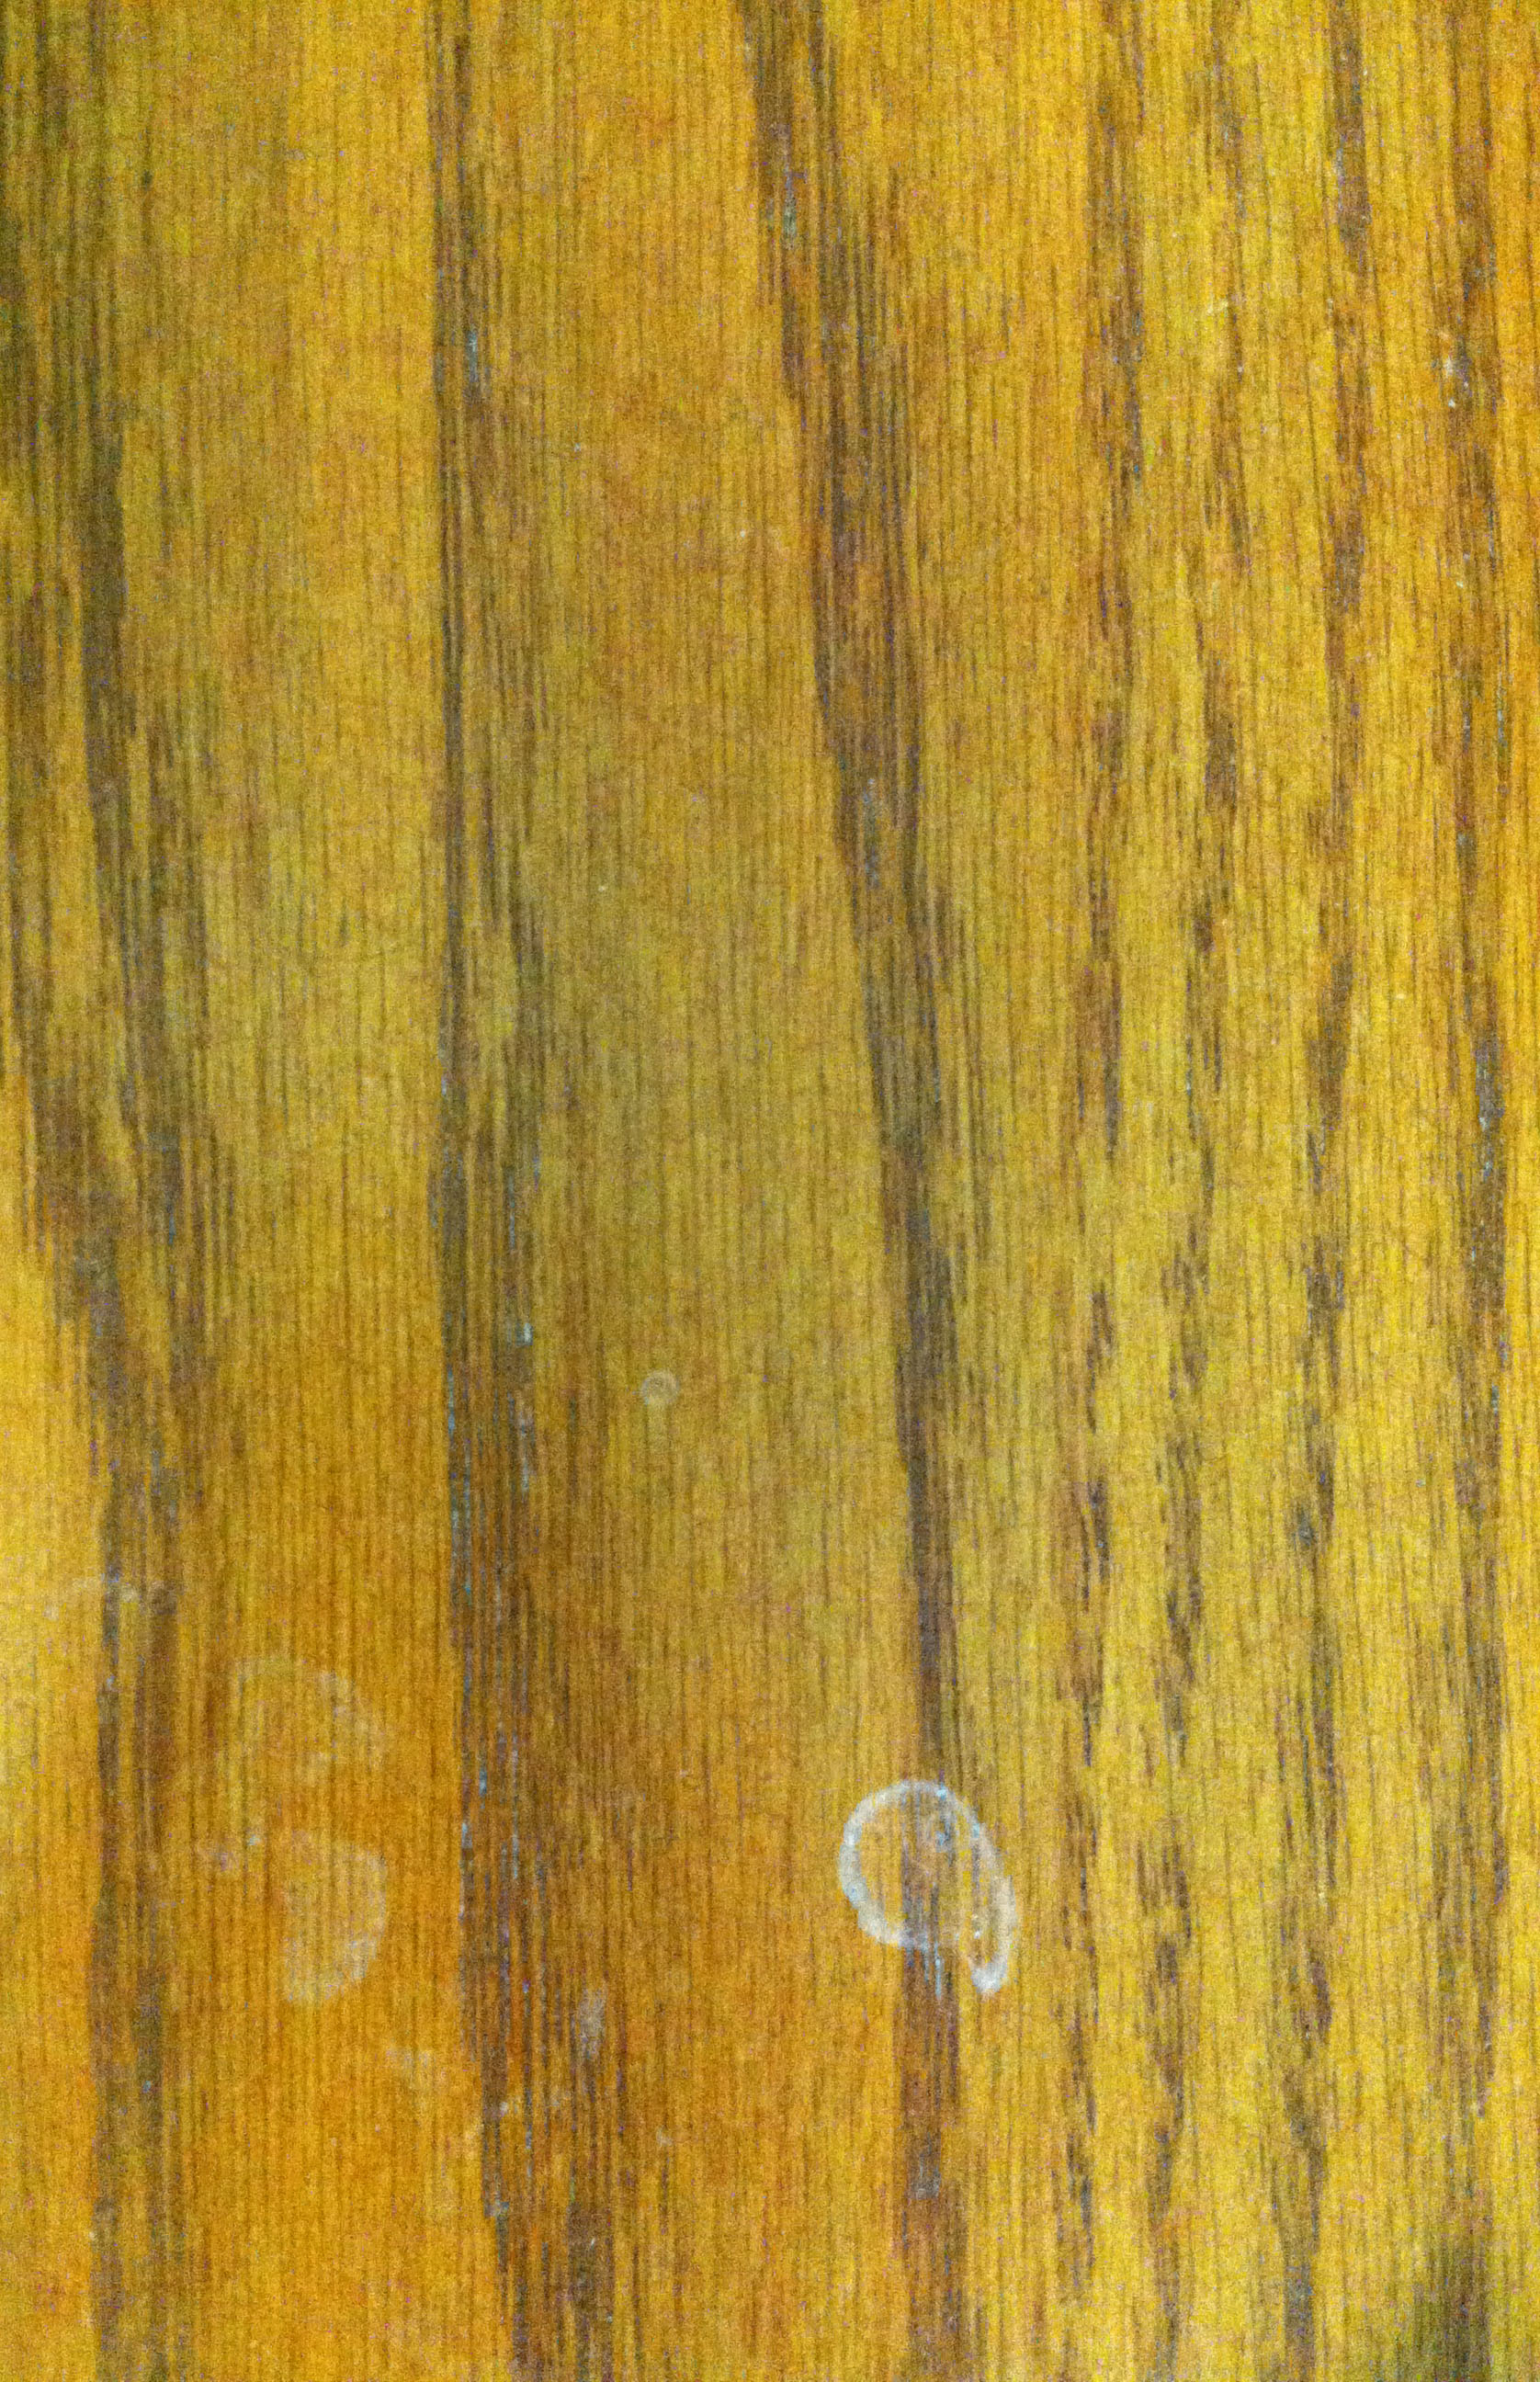
\includegraphics[height=2in]{assets/segment_before.jpg}
\caption{Segmentation fail}
\label{fig:before_segment}
\end{figure}

\subsection{Window}
Through experimentation it was qualitatively determined that in general the window approach performed more accurately than the initial segmentation approach. Figure~\ref{fig:red_window} shows the result of running the window algorithm on a stain. While the window approach performed better than the segmentation approach, the results still varied on an image by image basis. Certain parameters of the algorithm could be adjusted to improve performance but the adjustments varied between pictures and cannot be set automatically. Table~\ref{table:window_table} displays the statistical results of the window detection approach. One thing to note is that the recall rate may not accurately reflect true values since they were calculated based on windows. A higher recall on larger windows is misleading since a stain might only encompass only part of the window.

\begin{table}[!ht]
\begin{center} \begin{tabular}{l|c|r}
Window Size & Average Precision & Average Recall \\
\hline
5 & 0.640206848 & 0.161015766 \\
10 & 0.625077057 & 0.203232955 \\
20 & 0.646491238 & 0.262179909 \\
50 & 0.645036666 & 0.405706819 \\
\end{tabular} \end{center}
\caption{Window Results}
\label{table:window_table}
\end{table}

\begin{figure}[!ht]
\centering
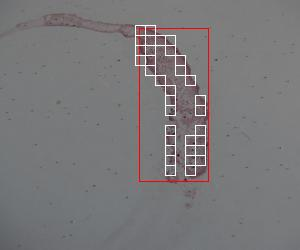
\includegraphics[height=2in]{assets/red-window.jpg}
% 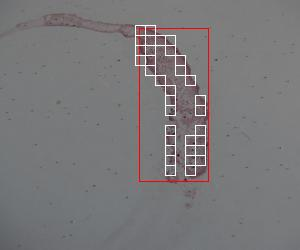
\epsfig{file=assets/red-window.jpg,width=1\columnwidth}
\caption{Window-based}
\label{fig:red_window}
\end{figure}

\subsection{SVM Learned}
The SVM implementation used in this paper was SVMlight~\cite{svm_light} and the window size is 10x10 for the examples used in this paper. Table~\ref{table:train1_test2} displays the result statistics of training on a sub-dataset labeled as ``dataset 1'' and testing on a sub-dataset labeled as ``dataset 2''. Table~\ref{table:train2_test1} displays the result statistics of the reciprocal training  and testing relationship. It is worth noting that the overall performance is higher in table~\ref{table:train2_test1} for multiple reasons. Dataset 1 is the first set of test images obtained and manually classified. The dataset contains images with slight contrast issues which leads to bad training data. This issue of contrast is further discussed later in this paper. Another reason for the poorer performance when training on dataset 1 results from misrepresentation of stains due to poor manual classification. Because most stains are not square in shape, attempting to classify curved stains using square bounding boxes will inevitably result in areas misclassified as stains. As a result, many pictures in the ``dataset 1'' contain misclassified examples and this source of error was noted before ``dataset 2'' was classified. The bounding boxes in ``dataset 2'' are drawn much closer to the shape of the stain in order to reduce error and the results show a definite reduction.

Qualitative comparisons between the SVM detected and window detected regions also highlight the improved performance brought on by machine learning. Figure~\ref{fig:coffee_comparison} shows the results of window-based detection on the left and the results of learning on the right. It is worth noting that not only does the learning approach label much more of the stain, it also correctly identifies sections of the stain that were not classified initially. Figure~\ref{fig:pattern_comparison} best highlights the advantages of the learning approach. In the top image, the window-based detector incorrectly identified the background pattern as a series of stains. In the bottom image the SVM correctly labels the stained region while not misclassifying the background pattern.

A parameter that must be specified when using a SVM is c, which determines the penalty for a misclassified instance. Testing on the validation set, we found that $c=0.0001$ generally gave good performance. This also correlates to a trade-off between recall and precision. By using a higher c, we trade higher recall for precision.

\subsection{Error Analysis}
Most of the cases where the SVM failed were in images where there are lighting differences or other artifacts that fit our original definition of a stain. Figure~\ref{fig:contrast_fail} shows a representative case of where our method fails. The image has major lighting differences which makes identifying the background difficult. This might be solved by first segmenting the image first and then applying the SVM on the individual segments. This will be explored for the following sprint.

\begin{table}
\begin{center} \begin{tabular}[h]{l|l|l|l}
c & Accuracy & Precision & Recall \\ 
\hline
0.00075 & 46.2 & 35.81 & 9.58 \\ 
0.001 & 50.71 & 51.88 & 19.55 \\ 
0.01 & 55.52 & 55.19 & 58.76 \\ 
0.1 & 45.67 & 46.77 & 62.69 \\ 
1 & 50.94 & 63.67 & 4.37 \\ 
10 & 49.02 & 48.71 & 36.99 \\ 
100 & 49.02 & 48.71 & 36.99 \\ 
1000 & 49.02 & 48.71 & 36.99 \\
\end{tabular} \end{center}
\caption{SVM Results from training on dataset 1 and testing on 2}
\label{table:train1_test2}
\end{table}

\begin{table}
\begin{center} \begin{tabular}[h]{l|l|l|l}
c & Accuracy & Precision & Recall \\
\hline
0.00075 & 66.12 & 72.74 & 51.62 \\
0.001 & 66.12 & 72.71 & 51.65 \\
0.01 & 66.12 & 72.77 & 51.59 \\
0.1 & 49.99 & 50.01 & 87.9 \\
1 & 50.19 & 50.15 & 70.8 \\
10 & 49.61 & 49.82 & 97.86 \\
100 & 56.28 & 54.26 & 80.15 \\
1000 & 56.28 & 54.26 & 80.15 \\
10000 & 56.28 & 54.26 & 80.15 \\
\end{tabular} \end{center}
\caption{SVM Results from training on dataset 2 and testing on 1}
\label{table:train2_test1}
\end{table}

\begin{figure*}[t]
\centering
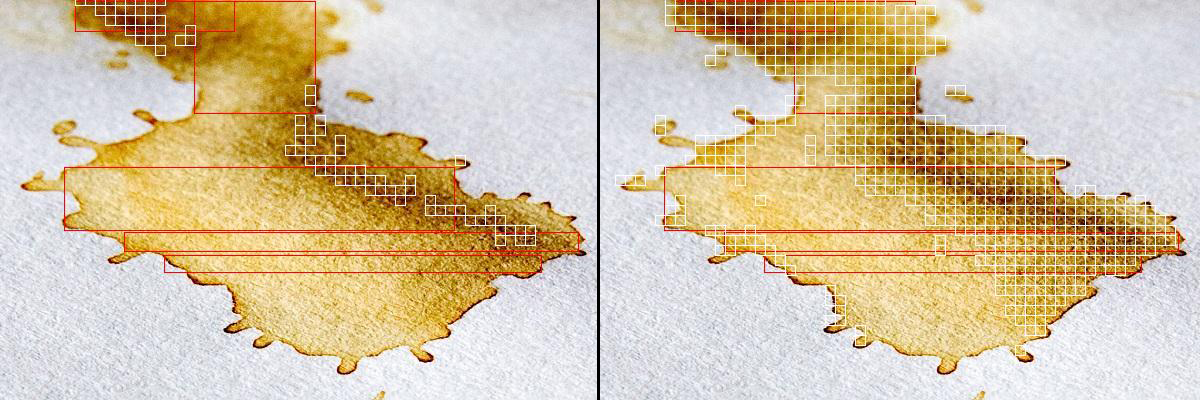
\epsfig{file=assets/coffee_window_vs_svm.png,width=2\columnwidth}
\caption{Comparison of window feature detection (left) and SVM detection (right)}
\label{fig:coffee_comparison}
\end{figure*}

\begin{figure}
\centering
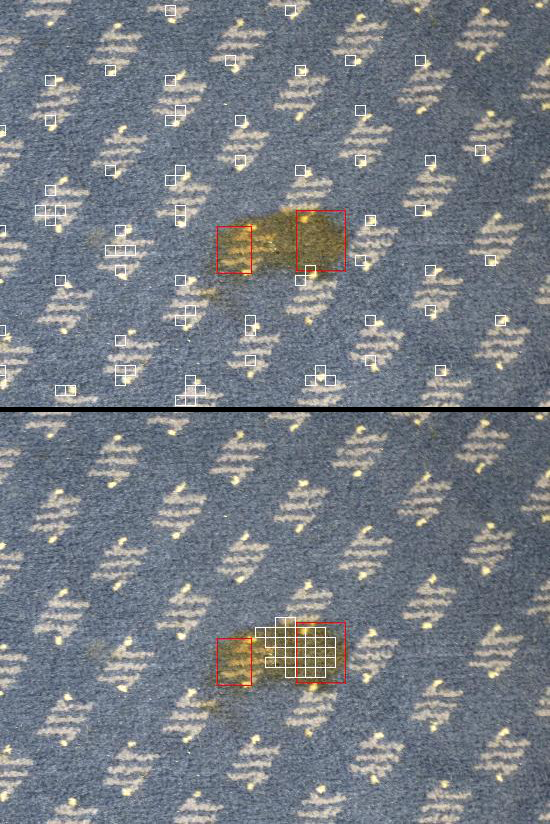
\includegraphics[height=3in]{assets/pattern_window_vs_svm.png}
% 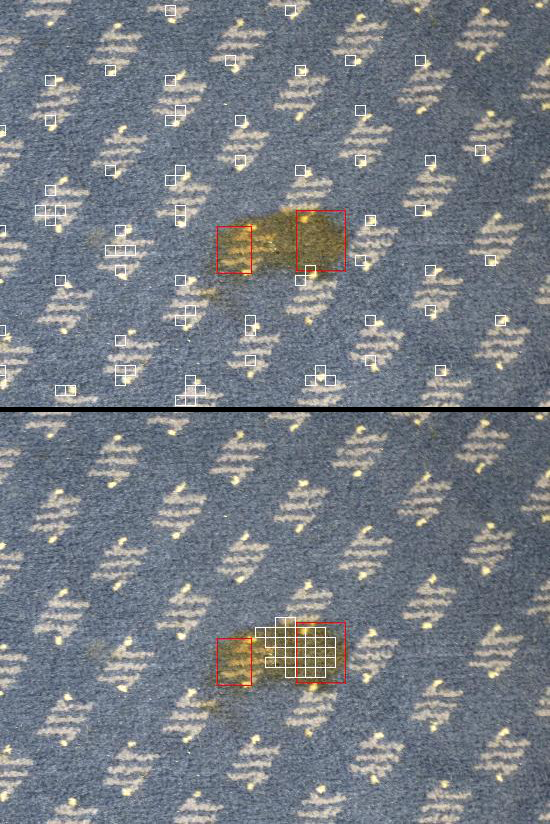
\epsfig{file=assets/pattern_window_vs_svm.png,width=1\columnwidth}
\caption{Comparison of window feature detection (left) and SVM detection (right)}
\label{fig:pattern_comparison}
\end{figure}


\begin{figure}
\centering

\includegraphics[height=2.5in]{assets/contrast_fail.jpg}
\caption{Bad Contrast}
\label{fig:contrast_fail}
\end{figure}

\subsection{Future Work}
While the learning approach towards stain detection has proven to be more effective than segmentation and window comparison-based solutions, the process could benefit from additional image preprocessing to reduce error. For example, erosion filters would remove small noise and dilation filters would strengthen stain connected components. An additional source of error reduction is better manual classification techniques. As noted in the results section there was a significant improvement in performance when manual classification techniques were improved. While the creation of a classification tool may be out of the scope of the project, we may work on it if there is additional time.


\begin{thebibliography}{99}

\bibitem{watershed} Serge Beucher and Christian Lantu�joul. Use of Watersheds in Contour Detection. In International workshop on image processing, real-time edge and motion detection (1979).

\bibitem{watershed_stackoverflow} Abid, K. (2012, July 11). stackoverflow Retrieved from http://stackoverflow.com/questions/11294859/how-to-define-the-markers-for-watershed-in-opencv/11438165

\bibitem{dirty_egg} Mertens, K. (2005). Dirt detection on brown eggs by means of color computer vision. Manuscript submitted for publication, Egg Quality and Incubation Research Group, , Available from US National Library of Medicine. (16335136)Retrieved from http://www.ncbi.nlm.nih.gov/pubmed/16335136 

\bibitem{svm_light} T. Joachims, Making large-Scale SVM Learning Practical. Advances in Kernel Methods - Support Vector Learning, B. Sch�lkopf and C. Burges and A. Smola (ed.), MIT-Press, 1999.


% \bibitem{c2} W.-K. Chen, Linear Networks and Systems (Book style).	Belmont, CA: Wadsworth, 1993, pp. 123�135.
% \bibitem{c3} H. Poor, An Introduction to Signal Detection and Estimation.   New York: Springer-Verlag, 1985, ch. 4.
% \bibitem{c4} B. Smith, �An approach to graphs of linear forms (Unpublished work style),� unpublished.
% \bibitem{c5} E. H. Miller, �A note on reflector arrays (Periodical style�Accepted for publication),� IEEE Trans. Antennas Propagat., to be publised.
% \bibitem{c6} J. Wang, �Fundamentals of erbium-doped fiber amplifiers arrays (Periodical style�Submitted for publication),� IEEE J. Quantum Electron., submitted for publication.
% \bibitem{c7} C. J. Kaufman, Rocky Mountain Research Lab., Boulder, CO, private communication, May 1995.
% \bibitem{c8} Y. Yorozu, M. Hirano, K. Oka, and Y. Tagawa, �Electron spectroscopy studies on magneto-optical media and plastic substrate interfaces(Translation Journals style),� IEEE Transl. J. Magn.Jpn., vol. 2, Aug. 1987, pp. 740�741 [Dig. 9th Annu. Conf. Magnetics Japan, 1982, p. 301].
% \bibitem{c9} M. Young, The Techincal Writers Handbook.  Mill Valley, CA: University Science, 1989.
% \bibitem{c10} J. U. Duncombe, �Infrared navigation�Part I: An assessment of feasibility (Periodical style),� IEEE Trans. Electron Devices, vol. ED-11, pp. 34�39, Jan. 1959.
% \bibitem{c11} S. Chen, B. Mulgrew, and P. M. Grant, �A clustering technique for digital communications channel equalization using radial basis function networks,� IEEE Trans. Neural Networks, vol. 4, pp. 570�578, July 1993.
% \bibitem{c12} R. W. Lucky, �Automatic equalization for digital communication,� Bell Syst. Tech. J., vol. 44, no. 4, pp. 547�588, Apr. 1965.
% \bibitem{c13} S. P. Bingulac, �On the compatibility of adaptive controllers (Published Conference Proceedings style),� in Proc. 4th Annu. Allerton Conf. Circuits and Systems Theory, New York, 1994, pp. 8�16.
% \bibitem{c14} G. R. Faulhaber, �Design of service systems with priority reservation,� in Conf. Rec. 1995 IEEE Int. Conf. Communications, pp. 3�8.
% \bibitem{c15} W. D. Doyle, �Magnetization reversal in films with biaxial anisotropy,� in 1987 Proc. INTERMAG Conf., pp. 2.2-1�2.2-6.
% \bibitem{c16} G. W. Juette and L. E. Zeffanella, �Radio noise currents n short sections on bundle conductors (Presented Conference Paper style),� presented at the IEEE Summer power Meeting, Dallas, TX, June 22�27, 1990, Paper 90 SM 690-0 PWRS.
% \bibitem{c17} J. G. Kreifeldt, �An analysis of surface-detected EMG as an amplitude-modulated noise,� presented at the 1989 Int. Conf. Medicine and Biological Engineering, Chicago, IL.
% \bibitem{c18} J. Williams, �Narrow-band analyzer (Thesis or Dissertation style),� Ph.D. dissertation, Dept. Elect. Eng., Harvard Univ., Cambridge, MA, 1993. 
% \bibitem{c19} N. Kawasaki, �Parametric study of thermal and chemical nonequilibrium nozzle flow,� M.S. thesis, Dept. Electron. Eng., Osaka Univ., Osaka, Japan, 1993.
% \bibitem{c20} J. P. Wilkinson, �Nonlinear resonant circuit devices (Patent style),� U.S. Patent 3 624 12, July 16, 1990. 

\end{thebibliography}




\end{document}
